\documentclass{article}
\usepackage[utf8]{inputenc}
\usepackage[spanish]{babel}
\usepackage{graphicx, graphics, float, fancyhdr, titling}
\usepackage{listings}
\usepackage[a4paper, total={6in, 9.5in}]{geometry}
\usepackage{fancyhdr}
\usepackage{hyperref}   %para que funcione addcontentsline debe ser la ultima que se cargue

%\setcounter{secnumdepth}{-2}       %Poner solo esto si no se quieren numero delante de las secciones y niveles inferiores.

\renewcommand{\footrulewidth}{0.4pt}
\title{
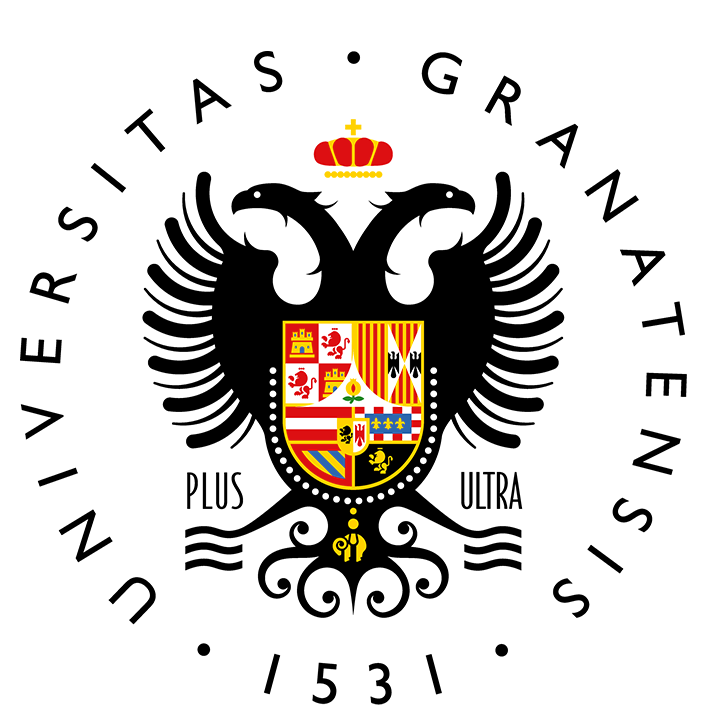
\includegraphics[width=1.75in]{imagenes/UGR-Logo.png} \\
\vspace*{1in}
\textbf{Cuestiones Tema 1} \\
Animación por Ordenador \\
\vspace*{0.5in}}
\author{Andrés Merlo Trujillo \\
andresmerlo@correo.ugr.es \\
77147239H \\ 
\vspace*{0.5in} \\
E.T.S. de Ingenierías Informática y de Telecomunicación \\
\textbf{Universidad de Granada}} \date{\today}

\hypersetup{
    colorlinks=true,
    linkcolor=black,
}

\renewcommand\maketitlehooka{\null\mbox{}\vfill}
\renewcommand\maketitlehookd{\vfill\null}

\begin{document}
\begin{titlingpage}
\maketitle
\end{titlingpage}

\tableofcontents

\newpage

\pagestyle{fancy}   %a partir de comienza el header (se salta el indice y portada)
\fancyhead[L]{Andrés Merlo Trujillo}
\fancyhead[R]{Animación por Ordenador}
%\section{Ejercicio 1}
%\begin{figure}[H]
%    \centering
%    \includegraphics[width=\textwidth]{imagenes/passwdfile.png}
%\end{figure}

\section{¿Qué es la animación?}

La animación es un proceso que permite dar la ilusión de movimiento a las imágenes, haciendo que se dé la ilusión de que la escena está cambiando. [WIKIPEDIA] 

\bigskip

Existen diversas técnicas de animación, pero todas ellas residen en el hecho de realizar múltiples imágenes con cambios ligeros y que se presentan de manera sucesiva de manera rápida y constante, dando la sensación de movimiento y que las cosas cambian (luz, forma, color, posición, etc.). Además, por norma general, se suelen usar 24 fotogramas por segundo para generar las animaciones (aunque también puede ser más alta, generando una sensación de movimiento más fluida). [TRANS]

\bigskip

A lo largo de la historia han existido diversos precursores de la animación, desde pinturas prehistóricas hasta proyecciones de imágenes. [TRANS]

\section{Buscad información sobre el fenómeno Phi e indicad la relación con la animación y lo comentado hasta ahora.}

El fenómeno phi, es una ilusión óptica que permite tener sensación de movimiento en donde hay imágenes estáticas que cambian a una frecuencia determinada [WIKIPEDIA2]. 

\bigskip

Todo esto se basa en la persistencia retiniana (o persistencia visual), que consiste en una limitación del ojo humano para procesar las imágenes a tanta velocidad, haciendo que se vea movimiento en esta sucesión [WIKIPEDIA3]. Esto hace que el cerebro interpole las imágenes para darles suavidad.

\bigskip

La relación con la animación se basa en estos dos conceptos, ya que sirven de ``herramienta'' básica para poder generar la sensación de movimiento esperado de las imágenes estáticas creadas para hacer la animación. 


\section{Busca información sobre antiguos artefactos que aplicaban la idea de persistencia visual}

A continuación voy a pasar a explicar como funcionaba cada artefacto mostrado en las transparencias.

\begin{itemize}
    \item \textbf{Linterna mágica: }Aparato óptico que consistía en un juego de lentes, con una cámara interna donde se colocaba la fuente de luz, y delante se colocaban las imágenes, que eran iluminadas y proyectadas a los espectadores. [WIKIPEDIA4] 
    
    Estas imágenes se pueden clasificar en distintos tipos, pero las que son útiles para la asignatura son las mecánicas. Por ejemplo, las \textit{Simple Slipping Slides} consistian en dos placas que mostraban dos momentos distintos y para hacer simular movimiento se cambiaba rapidamente a la otra placa.[WIKIPEDIA4]

    Otro sistema era el de uso de un disco con varias imágenes, que iba rotando y presentando las distintas imágenes para dar sensación de movimiento.

    Esto tiene que ver con la persistencia visual en el hecho de que se presentan dos imágenes lo suficientemente rápido como para dar sensación de movimiento; es decir, su funcionamiento se basa en este fenómeno si se quiere crear movimiento en las escenas.

    \item \textbf{Taumátropo: }Es un juguete consistente en un disco con dos imágenes distintas a ambos lado y una cuerda a cada lado del disco. Haciendo girar rápidamente el taumátropo, se genera la ilusión de que ambas imágenes están juntas. [WIKIPEDIA5]
    
    Los dibujos más comunes son un pájaro y una jaula, que al hacerlos girar da la sensación de que el pájaro está en dicha jaula.

    Este juguete tiene relación con la persistencia retiniana al mostrar una secuencia de imágenes rápidamente (en el caso de este juguete son dos imágenes), haciendo que se produzca dicho fenómeno y produciendo así que al seguir estando la imagen anterior en la retina, se fusionen ambas imágenes.

    \item \textbf{Kinetoscopio: }Precursor del proyector de películas, al hacer uso de una cinta para almacenar las imágenes. Sin embargo, no se podía proyectar en una pantalla, era solo para uso individual.[WIKIPEDIA6]
    
    Consistía en una caja en la que dentro se instalaba la cinta con todas las imágenes y de una fuente de luz con un obturador de luz de alta velocidad.[WIKIPEDIA6]

    Está relacionado con la persistencia visual al pasar rápidamente las imágenes de la cinta por el obturador, y dando la sensación de movimiento para aquella persona que esté observando por la lente.

    \item \textbf{Zoótropo: }Máquina estroboscópica, compuesta por un tambor circular con cortes y cuyo interior tiene imágenes secuenciales del movimiento de un objeto o escena. El observador tiene que mirar por las ranuras para poder observar las imágenes y poder apreciar el movimiento. Además, tiene la ventaja de que varias personas pueden usarlo a la vez.[WIKIPEDIA7]
    
    Tiene relación con la persistencia visual al mostrar las imágenes de manera rápida y continuada. Esto se consigue mediante las ranuras, que actúan de visor en el momento en el que se encuentran delante del espectador y cuando no estén delante desaparezca la imagen para que la siguiente ranura muestre la siguiente. Esto al final hace el efecto de que aparezca y desaparezca la imagen.
\end{itemize}


\section{Busca información sobre estas cuatro técnicas centrándote principalmente en las dos últimas}

Voy a dividir cada apartado en subsecciones.

\subsection{Rotoscopia}

La rotoscopia es una técnica de animación que los animadores utilizan consistente en dibujar las imágenes que componen una animación fotograma a fotograma, utilizando como base una grabación real de la animación que se desea dibujar. Antiguamente, se hacía uso del rotoscopio, que es una máquina que proyectaba la grabación en un panel de cristal y donde el dibujante calcaba el fotograma a dibujo. [https://en.wikipedia.org/wiki/Rotoscoping]

\bigskip

Algunos ejemplos de películas son \textit{Blancanieves y los siete enanitos}, \textit{Alicia en el país de las maravillas}. [https://soydecine.com/rotoscopia/] y \textit{Star Wars} para crear los sables láser [https://en.wikipedia.org/wiki/Rotoscoping]

\subsection{Animación paso a paso}

Técnica de animación consistente en la elaboración de imágenes individuales (cuadros) cuyo movimiento o cualquiera de los demás atributos varía ligeramente. Al ser un proceso manual, se suele tardar mucho más que con otras técnicas. Se crea la ilusión de movimiento al mostrar rápidamente dichas imágenes. 

\bigskip

Ha sido ampliamente utilizada para dibujos animados y programas de televisión. Hoy en día se suele realizar este tipo de animación mediante el ordenador. 

\bigskip

Un ejemplo de animación paso a paso es el \textit{Stop Motion}, en el que se fotografían escenas y personajes, y en cada fotograma se varía un poco para dar la sensación de movimiento al unirlas.


\subsection{Animación por claves}

Técnica utilizada para la animación digital y de películas. Consiste en definir puntos clave de una animación, indicando en dicho punto la posición, rotación, escala u otras propiedades. Después, mediante un software de animación (Blender, 3ds Max, etc.) se interpolan las posiciones intermedias entre estos puntos clave, creando una animación fluida. [https://www.adobe.com/creativecloud/video/discover/keyframing.html]

\bigskip

Además, se puede modificar la forma en la que se interpola dicha animación mediante funciones, haciendo que, por ejemplo, un objeto acelere hasta el siguiente punto clave, mantenga la velocidad, acelere y frene, vaya frenando o incluso modelar una función personalizada.

\bigskip

Por último, cabe destacar que este tipo de animación permite ahorrar al animador mucho tiempo, al no tener que animar fotograma a fotograma (animación paso a paso) los objetos. [https://www.adobe.com/creativecloud/video/discover/keyframing.html]


\subsection{Animación procedural}

Es una técnica de animación usada para generar automáticamente animaciones en tiempo real, permitiendo tener una serie de animaciones mucho más amplia que con las técnicas anteriores. %[https://en.wikipedia.org/wiki/Procedural_animation]

\bigskip

Normalmente es usado para generar sistemas de partículas (humo, agua, fuego, etc.), para la animación de la ropa de un personaje o el pelo del mismo. También se puede usar para dar realismo al mundo, al poder usarse para hacer sistemas de física \textit{ragdoll} (en inglés \textit{Ragdoll Physics}) [https://es.wikipedia.org/wiki/F%C3%ADsica_ragdoll]. 
Esto hace que las animaciones de muerte, por ejemplo, sean dinámicas y más realistas dependiendo de la situación en la que se encuentre el personaje, frente a la sensación de rigidez que puede dar las otras técnicas de animación, en las que dicha animación estaría predefinida.

\bigskip

Como desventaja se puede decir que tiene un mayor consumo de la CPU frente a las animaciones manuales, al tener que calcular el siguiente fotograma de la animación en tiempo real.
\end{document}
